\documentclass[12pt]{beamer}

%Preamble
\title{Latex Slides}
\author{Amanpreet Singh}
\date[Conf 2023] % (optional)
{Oct 25, 2023}
\institute[DPS] % (optional)
{
  \inst{1}
  Faculty of Physics\\
  Dashmesh Public School
  \and
  \inst{2}
  Faculty of Chemistry\\
  BNMIT
}

% Styling
\usetheme{CambridgeUS}
\usecolortheme{crane}
\usefonttheme{structuresmallcapsserif}
\hypersetup{
    colorlinks=true,
    linkcolor=blue,
    filecolor=magenta,      
    urlcolor=red,
    pdftitle={Latex Tutorial},
    pdfpagemode=FullScreen,
}

%Config
\graphicspath{{../../../../../common/images/stock/}}

\begin{document}
\maketitle

\begin{frame}
\frametitle{First Slide}
This is first Slide created with Latex and Beamer.\\
This has just the Normal Text.

Following \href{https://latex-beamer.com/tutorials/beamer-themes/}{Tutorial} for Basics of Latex and Beamer.
Another useful \href{https://www.overleaf.com/learn/latex/Beamer}{guide}.
\end{frame}

\begin{frame}
\frametitle{Themes}
Beamer has many \textbf{Themes} which can be specified in preamble.

\textbf{Theme Sources}
\begin{itemize}
    \item \href{https://deic.uab.cat/~iblanes/beamer_gallery/index_by_theme.html}{Theme Browser}
    \item \href{https://hartwork.org/beamer-theme-matrix/}{Theme Matrix} (Theme and Color)
\end{itemize}

\end{frame}

\begin{frame}
    \frametitle{Formatting}
    List Heading
    \begin{itemize}
        \item Content of this Slide.
        \item In Bullet Point format.
        \item It is very easy to Create.
        \item Wait before Next Section.\pause
    \end{itemize}

    \begin{alert}{Warning}
        Alert message !!
    \end{alert}

\end{frame}

\begin{frame}
    \frametitle{Blocks}
    
    \begin{alertblock}{Warning}
        Alert message in Alert Block !!
    \end{alertblock}
    
    \begin{exampleblock}{Example}
        Example message in Example Block ..
    \end{exampleblock}
    
    \begin{block}{Remark}
        Remark text
    \end{block}

\end{frame}

\begin{frame}
    \frametitle{Images}
    A Sail Boat ..
    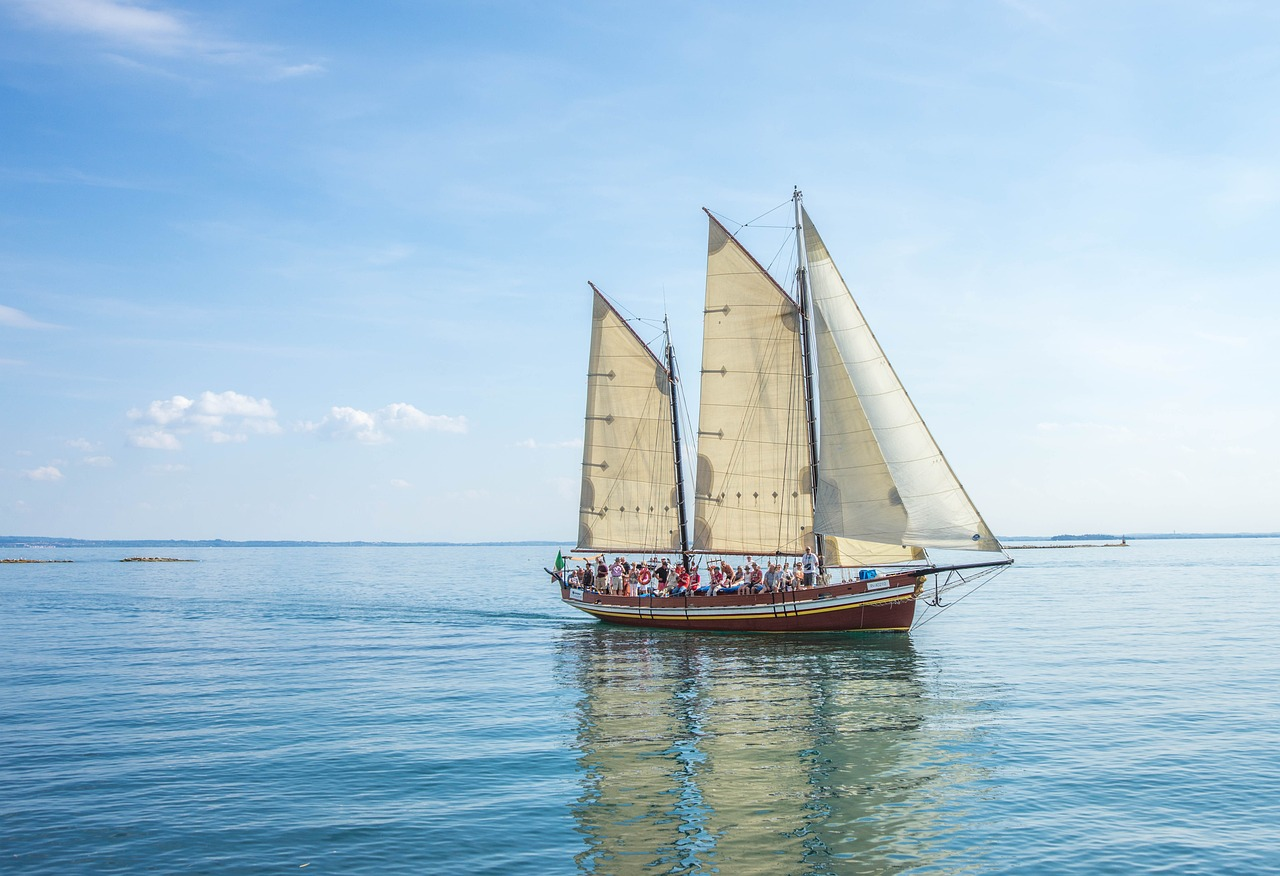
\includegraphics[width=0.8\linewidth]{boat.jpg}
\end{frame}

\begin{frame}
    \frametitle{Two-column slide}
    \begin{columns}
        \column{0.5\textwidth}
        This is a text in first column.
        $$E=mc^2$$
        \begin{itemize}
        \item First item
        \item Second item
        \end{itemize}
        
        \column{0.5\textwidth}
        This text will be in the second column
        and on a second thoughts, this is a nice looking
        layout in some cases.
        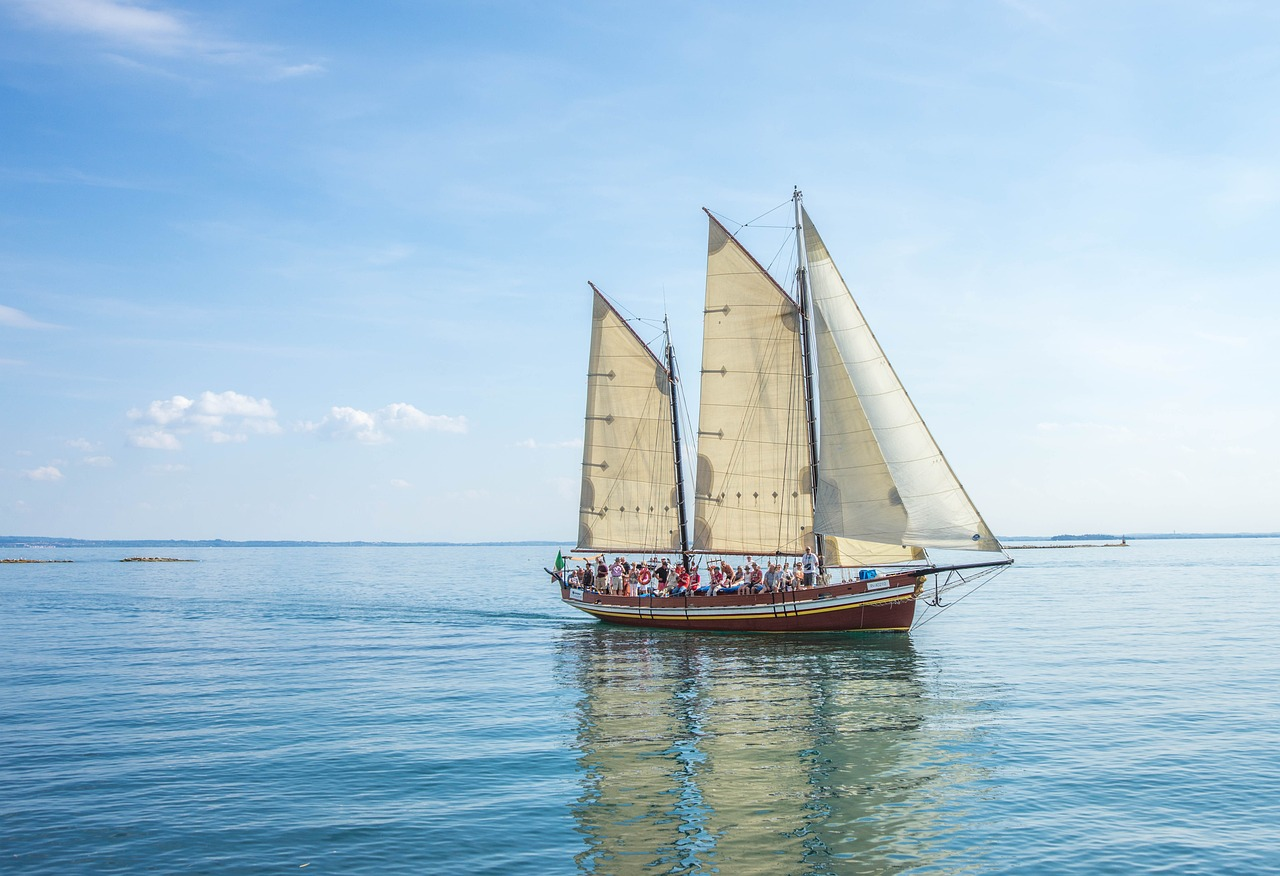
\includegraphics[width=0.8\linewidth]{boat.jpg}
    \end{columns}
\end{frame}

\end{document}